% Made up for the tikra benchmark.
\usepgfplotslibrary{dateplot}
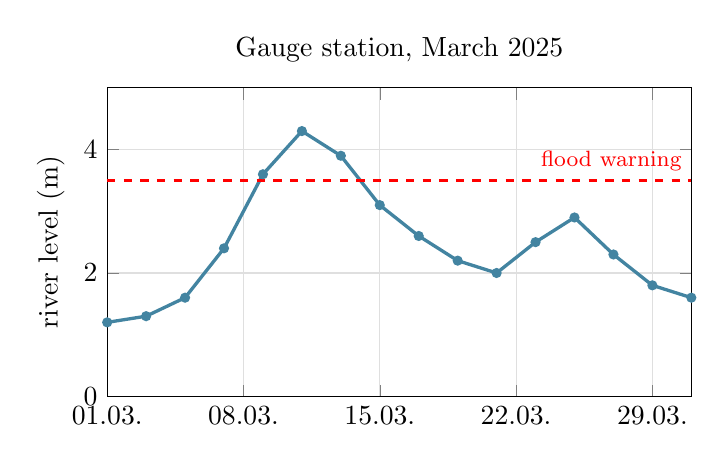
\begin{tikzpicture}
\begin{axis}[date coordinates in=x, date ZERO=2025-03-01,
    xticklabel=\day.\month., xtick={2025-03-01,2025-03-08,2025-03-15,2025-03-22,2025-03-29},
    xmin=2025-03-01, xmax=2025-03-31,
    ylabel={river level (m)}, ymin=0, ymax=5,
    width=9cm, height=5.5cm, grid=major, grid style={gray!25},
    title={Gauge station, March 2025}]
  \addplot[very thick, cyan!60!black, mark=*, mark size=1.2pt] coordinates {
    (2025-03-01,1.2) (2025-03-03,1.3) (2025-03-05,1.6) (2025-03-07,2.4)
    (2025-03-09,3.6) (2025-03-11,4.3) (2025-03-13,3.9) (2025-03-15,3.1)
    (2025-03-17,2.6) (2025-03-19,2.2) (2025-03-21,2.0) (2025-03-23,2.5)
    (2025-03-25,2.9) (2025-03-27,2.3) (2025-03-29,1.8) (2025-03-31,1.6)};
  \addplot[thick, red, dashed] coordinates {(2025-03-01,3.5) (2025-03-31,3.5)};
  \node[red, font=\footnotesize, above left] at (axis cs:2025-03-31,3.5) {flood warning};
\end{axis}
\end{tikzpicture}
